\appendix

\chapter{Demonstration of the interpreter modeling Pure Data\label{appendix:Pure-Data}}

\chaptermark{Pure Data interpreter}

%BEGIN LYX DEMO

To wrap up the presentation of the interpreter modeling Pure Data, we present
a demonstration of its use. We build a simple synthesizer with both frequency
and amplitude controllable via events, and use it to play a simple tune.
First, we define a few constants corresponding to the frequency in Hertz of
some musical notes:

\begin{hscode}\SaveRestoreHook
\column{B}{@{}>{\hspre}l<{\hspost}@{}}%
\column{9}{@{}>{\hspre}l<{\hspost}@{}}%
\column{E}{@{}>{\hspre}l<{\hspost}@{}}%
\>[B]{}\Varid{cSharp}{}\<[9]%
\>[9]{}\mathrel{=}\mathrm{554.37}{}\<[E]%
\\
\>[B]{}\Varid{aSharp}{}\<[9]%
\>[9]{}\mathrel{=}\mathrm{932.33}{}\<[E]%
\\
\>[B]{}\Varid{g}{}\<[9]%
\>[9]{}\mathrel{=}\mathrm{783.99}{}\<[E]%
\\
\>[B]{}\Varid{gSharp}{}\<[9]%
\>[9]{}\mathrel{=}\mathrm{830.61}{}\<[E]%
\\
\>[B]{}\Varid{f}{}\<[9]%
\>[9]{}\mathrel{=}\mathrm{698.46}{}\<[E]%
\ColumnHook
\end{hscode}\resethooks

Then, we construct the patch that corresponds to the following graph:

\begin{center}
\includegraphics[width=0.75\columnwidth]{puredata_example}
\par\end{center}

\begin{hscode}\SaveRestoreHook
\column{B}{@{}>{\hspre}l<{\hspost}@{}}%
\column{4}{@{}>{\hspre}l<{\hspost}@{}}%
\column{7}{@{}>{\hspre}l<{\hspost}@{}}%
\column{15}{@{}>{\hspre}l<{\hspost}@{}}%
\column{21}{@{}>{\hspre}l<{\hspost}@{}}%
\column{26}{@{}>{\hspre}l<{\hspost}@{}}%
\column{35}{@{}>{\hspre}l<{\hspost}@{}}%
\column{40}{@{}>{\hspre}l<{\hspost}@{}}%
\column{59}{@{}>{\hspre}l<{\hspost}@{}}%
\column{68}{@{}>{\hspre}l<{\hspost}@{}}%
\column{73}{@{}>{\hspre}l<{\hspost}@{}}%
\column{92}{@{}>{\hspre}l<{\hspost}@{}}%
\column{101}{@{}>{\hspre}l<{\hspost}@{}}%
\column{E}{@{}>{\hspre}l<{\hspost}@{}}%
\>[B]{}\Varid{example}\mathrel{=}\Conid{PdPatch}\;(\Varid{fromList}\;[\mskip1.5mu {}\<[E]%
\\
\>[B]{}\hsindent{4}{}\<[4]%
\>[4]{}\Conid{PdAtomBox}\;{}\<[15]%
\>[15]{}(\Conid{PdFloat}\;\mathrm{0}),\mbox{\onelinecomment  0}{}\<[E]%
\\
\>[B]{}\hsindent{4}{}\<[4]%
\>[4]{}\Conid{PdObj}\;{}\<[15]%
\>[15]{}[\mskip1.5mu \Conid{PdSymbol}\;\text{\tt \char34 osc\char126 \char34},\Conid{PdFloat}\;\Varid{gSharp}\mskip1.5mu]\;\mathrm{2}\;\mathrm{1},\mbox{\onelinecomment  1}{}\<[E]%
\\
\>[B]{}\hsindent{4}{}\<[4]%
\>[4]{}\Conid{PdMsgBox}\;{}\<[15]%
\>[15]{}[\mskip1.5mu \Conid{PdCmd}\;\Conid{PdToOutlet}\;(\Varid{map}\;(\Conid{PdTAtom}\mathbin{\circ}\Conid{PdFloat})\;[\mskip1.5mu \mathrm{0.5},\mathrm{1000}\mskip1.5mu])\mskip1.5mu],\mbox{\onelinecomment  2}{}\<[E]%
\\
\>[B]{}\hsindent{4}{}\<[4]%
\>[4]{}\Conid{PdMsgBox}\;{}\<[15]%
\>[15]{}[\mskip1.5mu \Conid{PdCmd}\;\Conid{PdToOutlet}\;(\Varid{map}\;(\Conid{PdTAtom}\mathbin{\circ}\Conid{PdFloat})\;[\mskip1.5mu \mathrm{0},\mathrm{100}\mskip1.5mu])\mskip1.5mu],\mbox{\onelinecomment  3}{}\<[E]%
\\
\>[B]{}\hsindent{4}{}\<[4]%
\>[4]{}\Conid{PdObj}\;{}\<[15]%
\>[15]{}[\mskip1.5mu \Conid{PdSymbol}\;\text{\tt \char34 line\char126 \char34}\mskip1.5mu]\;\mathrm{2}\;\mathrm{1},\mbox{\onelinecomment  4}{}\<[E]%
\\
\>[B]{}\hsindent{4}{}\<[4]%
\>[4]{}\Conid{PdObj}\;{}\<[15]%
\>[15]{}[\mskip1.5mu \Conid{PdSymbol}\;\text{\tt \char34 *\char126 \char34}\mskip1.5mu]\;\mathrm{2}\;\mathrm{1},\mbox{\onelinecomment  5}{}\<[E]%
\\
\>[B]{}\hsindent{4}{}\<[4]%
\>[4]{}\Conid{PdObj}\;{}\<[15]%
\>[15]{}[\mskip1.5mu \Conid{PdSymbol}\;\text{\tt \char34 dac\char126 \char34}\mskip1.5mu]\;\mathrm{1}\;\mathrm{0},\mbox{\onelinecomment  6}{}\<[E]%
\\[\blanklineskip]%
\>[B]{}\hsindent{4}{}\<[4]%
\>[4]{}\Conid{PdObj}\;{}\<[15]%
\>[15]{}[\mskip1.5mu \Conid{PdSymbol}\;\text{\tt \char34 receive\char34},\Conid{PdSymbol}\;\text{\tt \char34 MyMetro\char34}\mskip1.5mu]\;\mathrm{0}\;\mathrm{1},\mbox{\onelinecomment  7}{}\<[E]%
\\
\>[B]{}\hsindent{4}{}\<[4]%
\>[4]{}\Conid{PdObj}\;{}\<[15]%
\>[15]{}[\mskip1.5mu \Conid{PdSymbol}\;\text{\tt \char34 metro\char34},\Conid{PdFloat}\;\mathrm{500}\mskip1.5mu]\;\mathrm{2}\;\mathrm{1},\mbox{\onelinecomment  8}{}\<[E]%
\\
\>[B]{}\hsindent{4}{}\<[4]%
\>[4]{}\Conid{PdObj}\;{}\<[15]%
\>[15]{}[\mskip1.5mu \Conid{PdSymbol}\;\text{\tt \char34 delay\char34},\Conid{PdFloat}\;\mathrm{5}\mskip1.5mu]\;\mathrm{2}\;\mathrm{1},\mbox{\onelinecomment  9}{}\<[E]%
\\
\>[B]{}\hsindent{4}{}\<[4]%
\>[4]{}\Conid{PdObj}\;{}\<[15]%
\>[15]{}[\mskip1.5mu \Conid{PdSymbol}\;\text{\tt \char34 list\char34},\Conid{PdFloat}\;\mathrm{0.5},\Conid{PdFloat}\;\mathrm{0.1}\mskip1.5mu]\;\mathrm{2}\;\mathrm{1},\mbox{\onelinecomment  10}{}\<[E]%
\\
\>[B]{}\hsindent{4}{}\<[4]%
\>[4]{}\Conid{PdObj}\;{}\<[15]%
\>[15]{}[\mskip1.5mu \Conid{PdSymbol}\;\text{\tt \char34 list\char34},\Conid{PdFloat}\;\mathrm{0},\Conid{PdFloat}\;\mathrm{500}\mskip1.5mu]\;\mathrm{2}\;\mathrm{1},\mbox{\onelinecomment  11}{}\<[E]%
\\
\>[B]{}\hsindent{4}{}\<[4]%
\>[4]{}\Conid{PdObj}\;{}\<[15]%
\>[15]{}[\mskip1.5mu \Conid{PdSymbol}\;\text{\tt \char34 line\char126 \char34}\mskip1.5mu]\;\mathrm{1}\;\mathrm{1},\mbox{\onelinecomment  12}{}\<[E]%
\\
\>[B]{}\hsindent{4}{}\<[4]%
\>[4]{}\Conid{PdObj}\;{}\<[15]%
\>[15]{}[\mskip1.5mu \Conid{PdSymbol}\;\text{\tt \char34 osc\char126 \char34},\Conid{PdFloat}\;(\Varid{gSharp}\mathbin{/}\mathrm{2})\mskip1.5mu]\;\mathrm{1}\;\mathrm{1},\mbox{\onelinecomment  13}{}\<[E]%
\\
\>[B]{}\hsindent{4}{}\<[4]%
\>[4]{}\Conid{PdObj}\;{}\<[15]%
\>[15]{}[\mskip1.5mu \Conid{PdSymbol}\;\text{\tt \char34 *\char126 \char34}\mskip1.5mu]\;\mathrm{2}\;\mathrm{1},\mbox{\onelinecomment  14}{}\<[E]%
\\[\blanklineskip]%
\>[B]{}\hsindent{4}{}\<[4]%
\>[4]{}\Conid{PdMsgBox}\;{}\<[15]%
\>[15]{}[\mskip1.5mu \Conid{PdCmd}\;\Conid{PdToOutlet}\;{}\<[E]%
\\
\>[15]{}\hsindent{6}{}\<[21]%
\>[21]{}[\mskip1.5mu \Conid{PdTAtom}\;(\Conid{PdSymbol}\;\text{\tt \char34 list\char34}),\Conid{PdTAtom}\;(\Conid{PdSymbol}\;\text{\tt \char34 bang\char34})\mskip1.5mu]\mskip1.5mu],\mbox{\onelinecomment  15}{}\<[E]%
\\
\>[B]{}\hsindent{4}{}\<[4]%
\>[4]{}\Conid{PdMsgBox}\;{}\<[15]%
\>[15]{}[\mskip1.5mu \Conid{PdCmd}\;\Conid{PdToOutlet}\;{}\<[E]%
\\
\>[15]{}\hsindent{6}{}\<[21]%
\>[21]{}[\mskip1.5mu \Conid{PdTAtom}\;(\Conid{PdSymbol}\;\text{\tt \char34 list\char34}),\Conid{PdTAtom}\;(\Conid{PdSymbol}\;\text{\tt \char34 stop\char34})\mskip1.5mu]\mskip1.5mu],\mbox{\onelinecomment  16}{}\<[E]%
\\
\>[B]{}\hsindent{4}{}\<[4]%
\>[4]{}\Conid{PdMsgBox}\;{}\<[15]%
\>[15]{}[\mskip1.5mu \Conid{PdCmd}\;(\Conid{PdReceiver}\;\text{\tt \char34 MyMetro\char34})\;[\mskip1.5mu \Conid{PdTDollar}\;\mathrm{1}\mskip1.5mu]\mskip1.5mu]\mskip1.5mu]\mbox{\onelinecomment  17}{}\<[E]%
\\[\blanklineskip]%
\>[B]{}\hsindent{4}{}\<[4]%
\>[4]{})(\Varid{fromList}\;[\mskip1.5mu {}\<[E]%
\\
\>[4]{}\hsindent{3}{}\<[7]%
\>[7]{}((\mathrm{0},{}\<[26]%
\>[26]{}\mathrm{0})\rhd (\mathrm{1},{}\<[35]%
\>[35]{}\mathrm{0})),{}\<[40]%
\>[40]{}((\mathrm{1},{}\<[59]%
\>[59]{}\mathrm{0})\rhd (\mathrm{5},{}\<[68]%
\>[68]{}\mathrm{0})),{}\<[73]%
\>[73]{}((\mathrm{2},{}\<[92]%
\>[92]{}\mathrm{0})\rhd (\mathrm{4},{}\<[101]%
\>[101]{}\mathrm{0})),{}\<[E]%
\\
\>[4]{}\hsindent{3}{}\<[7]%
\>[7]{}((\mathrm{3},{}\<[26]%
\>[26]{}\mathrm{0})\rhd (\mathrm{4},{}\<[35]%
\>[35]{}\mathrm{0})),{}\<[40]%
\>[40]{}((\mathrm{4},{}\<[59]%
\>[59]{}\mathrm{0})\rhd (\mathrm{5},{}\<[68]%
\>[68]{}\mathrm{1})),{}\<[73]%
\>[73]{}((\mathrm{5},{}\<[92]%
\>[92]{}\mathrm{0})\rhd (\mathrm{6},{}\<[101]%
\>[101]{}\mathrm{0})),{}\<[E]%
\\
\>[4]{}\hsindent{3}{}\<[7]%
\>[7]{}((\mathrm{7},{}\<[26]%
\>[26]{}\mathrm{0})\rhd (\mathrm{8},{}\<[35]%
\>[35]{}\mathrm{0})),{}\<[40]%
\>[40]{}((\mathrm{8},{}\<[59]%
\>[59]{}\mathrm{0})\rhd (\mathrm{9},{}\<[68]%
\>[68]{}\mathrm{0})),{}\<[73]%
\>[73]{}((\mathrm{8},{}\<[92]%
\>[92]{}\mathrm{0})\rhd (\mathrm{10},{}\<[101]%
\>[101]{}\mathrm{0})),{}\<[E]%
\\
\>[4]{}\hsindent{3}{}\<[7]%
\>[7]{}((\mathrm{9},{}\<[26]%
\>[26]{}\mathrm{0})\rhd (\mathrm{11},{}\<[35]%
\>[35]{}\mathrm{0})),{}\<[40]%
\>[40]{}((\mathrm{10},{}\<[59]%
\>[59]{}\mathrm{0})\rhd (\mathrm{12},{}\<[68]%
\>[68]{}\mathrm{0})),{}\<[73]%
\>[73]{}((\mathrm{11},{}\<[92]%
\>[92]{}\mathrm{0})\rhd (\mathrm{12},{}\<[101]%
\>[101]{}\mathrm{0})),{}\<[E]%
\\
\>[4]{}\hsindent{3}{}\<[7]%
\>[7]{}((\mathrm{12},{}\<[26]%
\>[26]{}\mathrm{0})\rhd (\mathrm{14},{}\<[35]%
\>[35]{}\mathrm{0})),{}\<[40]%
\>[40]{}((\mathrm{13},{}\<[59]%
\>[59]{}\mathrm{0})\rhd (\mathrm{14},{}\<[68]%
\>[68]{}\mathrm{1})),{}\<[73]%
\>[73]{}((\mathrm{14},{}\<[92]%
\>[92]{}\mathrm{0})\rhd (\mathrm{6},{}\<[101]%
\>[101]{}\mathrm{0})),{}\<[E]%
\\
\>[4]{}\hsindent{3}{}\<[7]%
\>[7]{}((\mathrm{15},{}\<[26]%
\>[26]{}\mathrm{0})\rhd (\mathrm{17},{}\<[35]%
\>[35]{}\mathrm{0})),{}\<[40]%
\>[40]{}((\mathrm{16},{}\<[59]%
\>[59]{}\mathrm{0})\rhd (\mathrm{17},{}\<[68]%
\>[68]{}\mathrm{0}))\mskip1.5mu]{}\<[E]%
\\
\>[B]{}\hsindent{4}{}\<[4]%
\>[4]{})[\mskip1.5mu \mathrm{1},\mathrm{4},\mathrm{5},\mathrm{12},\mathrm{13},\mathrm{14},\mathrm{6}\mskip1.5mu]{}\<[E]%
\ColumnHook
\end{hscode}\resethooks

This is the sequence of input events that corresponds to playing the tune:

\begin{hscode}\SaveRestoreHook
\column{B}{@{}>{\hspre}l<{\hspost}@{}}%
\column{4}{@{}>{\hspre}l<{\hspost}@{}}%
\column{7}{@{}>{\hspre}l<{\hspost}@{}}%
\column{44}{@{}>{\hspre}l<{\hspost}@{}}%
\column{E}{@{}>{\hspre}l<{\hspost}@{}}%
\>[B]{}\Varid{main}\mathbin{::}\Conid{IO}\;(){}\<[E]%
\\
\>[B]{}\Varid{main}\mathrel{=}{}\<[E]%
\\
\>[B]{}\hsindent{4}{}\<[4]%
\>[4]{}\Varid{\Conid{ByteString}.putStr}\mathbin{\$}\Varid{runPut}\;(\Varid{putWav}\;\Varid{output}){}\<[E]%
\\
\>[B]{}\hsindent{4}{}\<[4]%
\>[4]{}\mathbf{where}{}\<[E]%
\\
\>[B]{}\hsindent{4}{}\<[4]%
\>[4]{}\Varid{output}\mathrel{=}\Varid{genOutput}\mathbin{\$}\Varid{runSteps}\;\mathrm{10000}\;\Varid{example}\;[\mskip1.5mu {}\<[E]%
\\
\>[4]{}\hsindent{3}{}\<[7]%
\>[7]{}(\Conid{PdEvent}\;\mathrm{1000}\;\mathrm{15}\;[\mskip1.5mu \Conid{PdSymbol}\;\text{\tt \char34 bang\char34}\mskip1.5mu]),\mbox{\onelinecomment  MyMetro bang}{}\<[E]%
\\
\>[4]{}\hsindent{3}{}\<[7]%
\>[7]{}(\Conid{PdEvent}\;\mathrm{1010}\;\mathrm{2}\;[\mskip1.5mu \Conid{PdSymbol}\;\text{\tt \char34 bang\char34}\mskip1.5mu]),{}\<[44]%
\>[44]{}\mbox{\onelinecomment  0.1 1000}{}\<[E]%
\\
\>[4]{}\hsindent{3}{}\<[7]%
\>[7]{}(\Conid{PdEvent}\;\mathrm{1900}\;\mathrm{3}\;[\mskip1.5mu \Conid{PdSymbol}\;\text{\tt \char34 bang\char34}\mskip1.5mu]),\mbox{\onelinecomment  0 100}{}\<[E]%
\\
\>[4]{}\hsindent{3}{}\<[7]%
\>[7]{}(\Conid{PdEvent}\;\mathrm{2001}\;\mathrm{0}\;[\mskip1.5mu \Conid{PdSymbol}\;\text{\tt \char34 float\char34},\Conid{PdFloat}\;\Varid{cSharp}\mskip1.5mu]),{}\<[E]%
\\
\>[4]{}\hsindent{3}{}\<[7]%
\>[7]{}(\Conid{PdEvent}\;\mathrm{2002}\;\mathrm{2}\;[\mskip1.5mu \Conid{PdSymbol}\;\text{\tt \char34 bang\char34}\mskip1.5mu]),{}\<[44]%
\>[44]{}\mbox{\onelinecomment  0.1 1000}{}\<[E]%
\\[\blanklineskip]%
\>[4]{}\hsindent{3}{}\<[7]%
\>[7]{}(\Conid{PdEvent}\;\mathrm{2900}\;\mathrm{3}\;[\mskip1.5mu \Conid{PdSymbol}\;\text{\tt \char34 bang\char34}\mskip1.5mu]),\mbox{\onelinecomment  0 100}{}\<[E]%
\\
\>[4]{}\hsindent{3}{}\<[7]%
\>[7]{}(\Conid{PdEvent}\;\mathrm{3001}\;\mathrm{0}\;[\mskip1.5mu \Conid{PdSymbol}\;\text{\tt \char34 float\char34},\Conid{PdFloat}\;\Varid{g}\mskip1.5mu]),{}\<[E]%
\\
\>[4]{}\hsindent{3}{}\<[7]%
\>[7]{}(\Conid{PdEvent}\;\mathrm{3002}\;\mathrm{2}\;[\mskip1.5mu \Conid{PdSymbol}\;\text{\tt \char34 bang\char34}\mskip1.5mu]),{}\<[44]%
\>[44]{}\mbox{\onelinecomment  0.1 1000}{}\<[E]%
\\[\blanklineskip]%
\>[4]{}\hsindent{3}{}\<[7]%
\>[7]{}(\Conid{PdEvent}\;\mathrm{4660}\;\mathrm{3}\;[\mskip1.5mu \Conid{PdSymbol}\;\text{\tt \char34 bang\char34}\mskip1.5mu]),\mbox{\onelinecomment  0 100}{}\<[E]%
\\
\>[4]{}\hsindent{3}{}\<[7]%
\>[7]{}(\Conid{PdEvent}\;\mathrm{4749}\;\mathrm{2}\;[\mskip1.5mu \Conid{PdSymbol}\;\text{\tt \char34 bang\char34}\mskip1.5mu]),{}\<[44]%
\>[44]{}\mbox{\onelinecomment  0.1 1000}{}\<[E]%
\\[\blanklineskip]%
\>[4]{}\hsindent{3}{}\<[7]%
\>[7]{}(\Conid{PdEvent}\;\mathrm{4750}\;\mathrm{0}\;[\mskip1.5mu \Conid{PdSymbol}\;\text{\tt \char34 float\char34},\Conid{PdFloat}\;\Varid{gSharp}\mskip1.5mu]),{}\<[E]%
\\
\>[4]{}\hsindent{3}{}\<[7]%
\>[7]{}(\Conid{PdEvent}\;\mathrm{4875}\;\mathrm{0}\;[\mskip1.5mu \Conid{PdSymbol}\;\text{\tt \char34 float\char34},\Conid{PdFloat}\;\Varid{aSharp}\mskip1.5mu]),{}\<[E]%
\\
\>[4]{}\hsindent{3}{}\<[7]%
\>[7]{}(\Conid{PdEvent}\;\mathrm{5000}\;\mathrm{0}\;[\mskip1.5mu \Conid{PdSymbol}\;\text{\tt \char34 float\char34},\Conid{PdFloat}\;\Varid{gSharp}\mskip1.5mu]),{}\<[E]%
\\[\blanklineskip]%
\>[4]{}\hsindent{3}{}\<[7]%
\>[7]{}(\Conid{PdEvent}\;\mathrm{5333}\;\mathrm{0}\;[\mskip1.5mu \Conid{PdSymbol}\;\text{\tt \char34 float\char34},\Conid{PdFloat}\;\Varid{f}\mskip1.5mu]),{}\<[E]%
\\[\blanklineskip]%
\>[4]{}\hsindent{3}{}\<[7]%
\>[7]{}(\Conid{PdEvent}\;\mathrm{5666}\;\mathrm{0}\;[\mskip1.5mu \Conid{PdSymbol}\;\text{\tt \char34 float\char34},\Conid{PdFloat}\;\Varid{cSharp}\mskip1.5mu]),{}\<[E]%
\\[\blanklineskip]%
\>[4]{}\hsindent{3}{}\<[7]%
\>[7]{}(\Conid{PdEvent}\;\mathrm{6000}\;\mathrm{0}\;[\mskip1.5mu \Conid{PdSymbol}\;\text{\tt \char34 float\char34},\Conid{PdFloat}\;\Varid{g}\mskip1.5mu]),{}\<[E]%
\\[\blanklineskip]%
\>[4]{}\hsindent{3}{}\<[7]%
\>[7]{}(\Conid{PdEvent}\;\mathrm{6650}\;\mathrm{3}\;[\mskip1.5mu \Conid{PdSymbol}\;\text{\tt \char34 bang\char34}\mskip1.5mu]),\mbox{\onelinecomment  0 100}{}\<[E]%
\\
\>[4]{}\hsindent{3}{}\<[7]%
\>[7]{}(\Conid{PdEvent}\;\mathrm{6745}\;\mathrm{2}\;[\mskip1.5mu \Conid{PdSymbol}\;\text{\tt \char34 bang\char34}\mskip1.5mu]),{}\<[44]%
\>[44]{}\mbox{\onelinecomment  0.1 1000}{}\<[E]%
\\[\blanklineskip]%
\>[4]{}\hsindent{3}{}\<[7]%
\>[7]{}(\Conid{PdEvent}\;\mathrm{6750}\;\mathrm{0}\;[\mskip1.5mu \Conid{PdSymbol}\;\text{\tt \char34 float\char34},\Conid{PdFloat}\;\Varid{gSharp}\mskip1.5mu]),{}\<[E]%
\\
\>[4]{}\hsindent{3}{}\<[7]%
\>[7]{}(\Conid{PdEvent}\;\mathrm{6875}\;\mathrm{0}\;[\mskip1.5mu \Conid{PdSymbol}\;\text{\tt \char34 float\char34},\Conid{PdFloat}\;\Varid{aSharp}\mskip1.5mu]),{}\<[E]%
\\
\>[4]{}\hsindent{3}{}\<[7]%
\>[7]{}(\Conid{PdEvent}\;\mathrm{7000}\;\mathrm{0}\;[\mskip1.5mu \Conid{PdSymbol}\;\text{\tt \char34 float\char34},\Conid{PdFloat}\;\Varid{gSharp}\mskip1.5mu]),{}\<[E]%
\\[\blanklineskip]%
\>[4]{}\hsindent{3}{}\<[7]%
\>[7]{}(\Conid{PdEvent}\;\mathrm{7000}\;\mathrm{16}\;[\mskip1.5mu \Conid{PdSymbol}\;\text{\tt \char34 bang\char34}\mskip1.5mu]),\mbox{\onelinecomment  MyMetro stop}{}\<[E]%
\\[\blanklineskip]%
\>[4]{}\hsindent{3}{}\<[7]%
\>[7]{}(\Conid{PdEvent}\;\mathrm{8000}\;\mathrm{3}\;[\mskip1.5mu \Conid{PdSymbol}\;\text{\tt \char34 bang\char34}\mskip1.5mu])\mskip1.5mu]\mbox{\onelinecomment  0 100}{}\<[E]%
\ColumnHook
\end{hscode}\resethooks

In Pure Data, the sound card is represented by the \texttt{dac\textasciitilde{}} object. Our
interpreter does nat handle actual audio output natively, but we can extract
the inlet data from that node from the list of states, and convert it to an
audio \texttt{wav} file format, that is then sent to standard output.

\begin{hscode}\SaveRestoreHook
\column{B}{@{}>{\hspre}l<{\hspost}@{}}%
\column{4}{@{}>{\hspre}l<{\hspost}@{}}%
\column{7}{@{}>{\hspre}l<{\hspost}@{}}%
\column{13}{@{}>{\hspre}l<{\hspost}@{}}%
\column{22}{@{}>{\hspre}l<{\hspost}@{}}%
\column{E}{@{}>{\hspre}l<{\hspost}@{}}%
\>[B]{}\Varid{convertData}\mathbin{::}\Conid{PdNodeState}\to [\mskip1.5mu \Conid{Integer}\mskip1.5mu]{}\<[E]%
\\
\>[B]{}\Varid{convertData}\;(\Conid{PdNodeState}\;\Varid{ins}\;\anonymous )\mathrel{=}{}\<[E]%
\\
\>[B]{}\hsindent{4}{}\<[4]%
\>[4]{}\mathbf{let}\;\Varid{inlet}\mathrel{=}\Varid{index}\;\Varid{ins}\;\mathrm{0}{}\<[E]%
\\
\>[B]{}\hsindent{4}{}\<[4]%
\>[4]{}\mathbf{in}\;\Varid{map}\;(\lambda (\Conid{PdFloat}\;\Varid{f})\to \Varid{floor}\;(\Varid{f}\mathbin{*}\mathrm{32768}))\;\Varid{inlet}{}\<[E]%
\\[\blanklineskip]%
\>[B]{}\Varid{everyOther}\mathbin{::}[\mskip1.5mu \Varid{a}\mskip1.5mu]\to [\mskip1.5mu \Varid{a}\mskip1.5mu]{}\<[E]%
\\
\>[B]{}\Varid{everyOther}\;(\Varid{x}\mathbin{:}(\Varid{y}\mathbin{:}\Varid{xs}))\mathrel{=}\Varid{x}\mathbin{:}\Varid{everyOther}\;\Varid{xs}{}\<[E]%
\\
\>[B]{}\Varid{everyOther}\;\Varid{x}\mathrel{=}\Varid{x}{}\<[E]%
\\[\blanklineskip]%
\>[B]{}\Varid{genOutput}\;\Varid{x}\mathrel{=}\Varid{concat}\mathbin{\$}\Varid{everyOther}{}\<[E]%
\\
\>[B]{}\hsindent{22}{}\<[22]%
\>[22]{}\mathbin{\$}\Varid{toList}{}\<[E]%
\\
\>[B]{}\hsindent{22}{}\<[22]%
\>[22]{}\mathbin{\$}\Varid{fmap}\;(\lambda (\Conid{PdState}\;\anonymous \;\Varid{nss}\;\anonymous \;\anonymous )\to \Varid{convertData}\mathbin{\$}\Varid{index}\;\Varid{nss}\;\mathrm{6})\;\Varid{x}{}\<[E]%
\\[\blanklineskip]%
\>[B]{}\Varid{putWav}\;\Varid{vs}\mathrel{=}{}\<[E]%
\\
\>[B]{}\hsindent{4}{}\<[4]%
\>[4]{}\mathbf{let}{}\<[E]%
\\
\>[4]{}\hsindent{3}{}\<[7]%
\>[7]{}\Varid{riff}{}\<[13]%
\>[13]{}\mathrel{=}\mathrm{0}\;\Varid{x46464952}{}\<[E]%
\\
\>[4]{}\hsindent{3}{}\<[7]%
\>[7]{}\Varid{wave}{}\<[13]%
\>[13]{}\mathrel{=}\mathrm{0}\;\Varid{x45564157}{}\<[E]%
\\
\>[4]{}\hsindent{3}{}\<[7]%
\>[7]{}\Varid{fmts}{}\<[13]%
\>[13]{}\mathrel{=}\mathrm{0}\;\Varid{x20746d66}{}\<[E]%
\\
\>[4]{}\hsindent{3}{}\<[7]%
\>[7]{}\Varid{datx}{}\<[13]%
\>[13]{}\mathrel{=}\mathrm{0}\;\Varid{x61746164}{}\<[E]%
\\
\>[4]{}\hsindent{3}{}\<[7]%
\>[7]{}\Varid{formatHeaderLen}\mathrel{=}\mathrm{16}{}\<[E]%
\\
\>[4]{}\hsindent{3}{}\<[7]%
\>[7]{}\Varid{fileSize}\mathrel{=}(\mathrm{44}\mathbin{+}(\Varid{length}\;\Varid{vs})\mathbin{*}\mathrm{2}){}\<[E]%
\\
\>[4]{}\hsindent{3}{}\<[7]%
\>[7]{}\Varid{bitsPerSample}\mathrel{=}\mathrm{16}{}\<[E]%
\\
\>[4]{}\hsindent{3}{}\<[7]%
\>[7]{}\Varid{format}\mathrel{=}\mathrm{1}{}\<[E]%
\\
\>[4]{}\hsindent{3}{}\<[7]%
\>[7]{}\Varid{channels}\mathrel{=}\mathrm{1}{}\<[E]%
\\
\>[4]{}\hsindent{3}{}\<[7]%
\>[7]{}\Varid{sampleRate}\mathrel{=}\mathrm{32000}{}\<[E]%
\\
\>[B]{}\hsindent{4}{}\<[4]%
\>[4]{}\mathbf{in}\;\mathbf{do}{}\<[E]%
\\
\>[4]{}\hsindent{3}{}\<[7]%
\>[7]{}\Varid{putWord32le}\;\Varid{riff}{}\<[E]%
\\
\>[4]{}\hsindent{3}{}\<[7]%
\>[7]{}\Varid{putWord32le}\;(\Varid{fromIntegral}\;\Varid{fileSize}){}\<[E]%
\\
\>[4]{}\hsindent{3}{}\<[7]%
\>[7]{}\Varid{putWord32le}\;\Varid{wave}{}\<[E]%
\\
\>[4]{}\hsindent{3}{}\<[7]%
\>[7]{}\Varid{putWord32le}\;\Varid{fmts}{}\<[E]%
\\
\>[4]{}\hsindent{3}{}\<[7]%
\>[7]{}\Varid{putWord32le}\;\Varid{formatHeaderLen}{}\<[E]%
\\
\>[4]{}\hsindent{3}{}\<[7]%
\>[7]{}\Varid{putWord16le}\;\Varid{format}{}\<[E]%
\\
\>[4]{}\hsindent{3}{}\<[7]%
\>[7]{}\Varid{putWord16le}\;\Varid{channels}{}\<[E]%
\\
\>[4]{}\hsindent{3}{}\<[7]%
\>[7]{}\Varid{putWord32le}\;\Varid{sampleRate}{}\<[E]%
\\
\>[4]{}\hsindent{3}{}\<[7]%
\>[7]{}\Varid{putWord32le}\;(\Varid{sampleRate}\mathbin{*}\Varid{bitsPerSample}\mathbin{*}(\Varid{fromIntegral}\;\Varid{channels})\mathbin{\Varid{`div`}}\mathrm{8}){}\<[E]%
\\
\>[4]{}\hsindent{3}{}\<[7]%
\>[7]{}\Varid{putWord16le}\;(((\Varid{fromIntegral}\;\Varid{bitsPerSample})\mathbin{*}\Varid{channels})\mathbin{\Varid{`div`}}\mathrm{8}){}\<[E]%
\\
\>[4]{}\hsindent{3}{}\<[7]%
\>[7]{}\Varid{putWord16le}\;(\Varid{fromIntegral}\;\Varid{bitsPerSample}){}\<[E]%
\\
\>[4]{}\hsindent{3}{}\<[7]%
\>[7]{}\Varid{putWord32le}\;\Varid{datx}{}\<[E]%
\\
\>[4]{}\hsindent{3}{}\<[7]%
\>[7]{}\Varid{putWord32le}\;(\Varid{fromIntegral}\;((\Varid{length}\;\Varid{vs})\mathbin{*}\mathrm{2})){}\<[E]%
\\
\>[4]{}\hsindent{3}{}\<[7]%
\>[7]{}\Varid{mapM\char95 }\;(\Varid{putWord16le}\mathbin{\circ}\Varid{fromIntegral})\;\Varid{vs}{}\<[E]%
\ColumnHook
\end{hscode}\resethooks

%END LYX DEMO


\chapter{Demonstration of the spreadsheet interpreter\label{appendix:Spreadsheet}}

\chaptermark{Spreadsheet interpreter}

We present here a demonstration of the spreadsheet interpreter in
use. This appendix is a Literate Haskell program including the complete
source code of the demonstration.

This program imports the interpreter defined in Chapter \ref{chap:Spreadsheets}
as a module, as well as some standard modules from the Haskell Platform.
We also use one additional module for tabular pretty-printing of the
output: \texttt{Text.PrettyPrint.Boxes}, available from Hackage, the
Haskell community's package repository\footnote{\url{https://hackage.haskell.org/package/boxes}}.

%BEGIN LYX DEMO

\begin{hscode}\SaveRestoreHook
\column{B}{@{}>{\hspre}l<{\hspost}@{}}%
\column{E}{@{}>{\hspre}l<{\hspost}@{}}%
\>[B]{}\mathbf{import}\;\Conid{XlInterpreter}{}\<[E]%
\\
\>[B]{}\mathbf{import}\;\Conid{\Conid{Data}.Char}\;(\Varid{chr},\Varid{ord}){}\<[E]%
\\
\>[B]{}\mathbf{import}\;\Conid{\Conid{Data}.\Conid{Map}.Strict}\;\Varid{as}\;\Conid{Map}\;(\Varid{foldlWithKey},\Varid{empty},\Varid{lookup},\Varid{toList},(\mathbin{!})){}\<[E]%
\\
\>[B]{}\mathbf{import}\;\Conid{\Conid{Text}.\Conid{PrettyPrint}.Boxes}\;\Varid{as}\;\Conid{Box}\;(\Varid{render},\Varid{hcat},\Varid{vcat},\Varid{text}){}\<[E]%
\\
\>[B]{}\mathbf{import}\;\Conid{\Conid{Text}.\Conid{PrettyPrint}.Boxes}\;\Varid{as}\;\Conid{Alignment}\;(\Varid{left},\Varid{right}){}\<[E]%
\ColumnHook
\end{hscode}\resethooks

Running the program produces the following output:

\begin{footnotesize}\begin{tabbing}\tt
~~~\char124{}A~~~~~~~~\char124{}B~~~~~~~~\char124{}C~~~~~~~~\char124{}D~~~~~~~~\char124{}E~~~~~~~~\char124{}F~~~~~~~~\char124{}G~~~~~~~~\\
\tt ~~1\char124{}~~~~~~~15\char124{}~~~~~~~15\char124{}\char34{}B\char34{}~~~~~~\char124{}~~~~~~~75\char124{}~~~~~~~30\char124{}~~~~~~105\char124{}~~~~~1015\\
\tt ~~2\char124{}~~~~~~~30\char124{}~~~~~~~15\char124{}~~~~~~~~1\char124{}~~~~~~~~~\char124{}~~~~~~~~~\char124{}~~~~~~~~~\char124{}~~~~~~~~~\\
\tt ~~3\char124{}~~~~~~~~~\char124{}~~~~~~~~~\char124{}~~~~~~~~~\char124{}~~~~~~~~~\char124{}~~~~~~~~~\char124{}~~~~~~~~~\char124{}~~~~~~~~~\\
\tt ~~4\char124{}~~~~~~~~~\char124{}~~~~~~~~~\char124{}~~~~~~~~~\char124{}~~~~~~~~~\char124{}~~~~~~~~~\char124{}~~~~~~~~~\char124{}~~~~~~~~~\\
\tt ~~5\char124{}~~~~~~~~~\char124{}~~~~~~~~~\char124{}\char34{}\char35{}VALUE\char33{}\char34{}\char124{}~~~~~~115\char124{}~~~~~~~~~\char124{}~~~~~~~15\char124{}~~~~~~~~~\\
\tt ~~6\char124{}~~~~~~~~~\char124{}~~~~~~~~~\char124{}~~~~~~~~~\char124{}~~~~~~130\char124{}~~~~~~~~~\char124{}~~~~~~~16\char124{}~~~~~~~~~\\
\tt ~~7\char124{}~~~~~~~~~\char124{}~~~~~~~~~\char124{}~~~~~~~~~\char124{}~~~~~~~~~\char124{}~~~~~~~~~\char124{}~~~~~~~~~\char124{}~~~~~~~~~\\
\tt ~~8\char124{}~~~~~~~~~\char124{}~~~~~~~~~\char124{}~~~~~~~~~\char124{}~~~~~~~~~\char124{}~~~~~~~~~\char124{}~~~~~~~~~\char124{}\char34{}\char35{}VALUE\char33{}\char34{}\\
\tt ~~9\char124{}~~~~~~~~~\char124{}~~~~~~~~~\char124{}~~~~~~~~~\char124{}~~~~~~~~~\char124{}~~~~~~~~~\char124{}~~~~~~~~~\char124{}~~~~~~~~~\\
\tt ~10\char124{}~~~~~~~10\char124{}~~~~~~~~~\char124{}~~~~~~~~~\char124{}~~~~~~~10\char124{}~~~~~~\char45{}20\char124{}~~~~~~~30\char124{}~~~~~~~~~\\
\tt ~11\char124{}\char34{}10\char34{}~~~~~\char124{}~~~~~~~~~\char124{}~~~~~~~~~\char124{}~~~~~~~~~\char124{}~~~~~~~20\char124{}~~~~~~~~~\char124{}~~~~~~~~~\\
\tt ~12\char124{}False~~~~\char124{}\char34{}\char35{}DIV\char47{}0\char33{}\char34{}\char124{}~~~~~~~~~\char124{}~~~~~~~~~\char124{}~~~~~~~~~\char124{}~~~~~~~~~\char124{}~~~~~~~~~\\
\tt ~13\char124{}True~~~~~\char124{}\char34{}\char35{}VALUE\char33{}\char34{}\char124{}~~~~~~~~~\char124{}~~~~~~~~~\char124{}~~~~~~~~~\char124{}~~~~~~~~~\char124{}~~~~~~~~~\\
\tt ~14\char124{}True~~~~~\char124{}\char34{}\char35{}DIV\char47{}0\char33{}\char34{}\char124{}~~~~~~~~~\char124{}~~~~~~~~~\char124{}~~~~~~~~~\char124{}~~~~~~~~~\char124{}~~~~~~~~~
\end{tabbing}
\end{footnotesize}


\section{Formatting}

In order to produce a more readable output, we define the instance \ensuremath{\Conid{Show}} for
our \ensuremath{\Conid{XlState}} type, using the \ensuremath{\Conid{\Conid{Text}.PrettyPrint}} package to produce tabular
outputs.

\begin{hscode}\SaveRestoreHook
\column{B}{@{}>{\hspre}l<{\hspost}@{}}%
\column{4}{@{}>{\hspre}l<{\hspost}@{}}%
\column{7}{@{}>{\hspre}l<{\hspost}@{}}%
\column{10}{@{}>{\hspre}l<{\hspost}@{}}%
\column{23}{@{}>{\hspre}c<{\hspost}@{}}%
\column{23E}{@{}l@{}}%
\column{26}{@{}>{\hspre}l<{\hspost}@{}}%
\column{28}{@{}>{\hspre}l<{\hspost}@{}}%
\column{35}{@{}>{\hspre}l<{\hspost}@{}}%
\column{45}{@{}>{\hspre}l<{\hspost}@{}}%
\column{E}{@{}>{\hspre}l<{\hspost}@{}}%
\>[B]{}\mathbf{instance}\;\Conid{Show}\;\Conid{XlState}\;\mathbf{where}{}\<[E]%
\\
\>[B]{}\hsindent{4}{}\<[4]%
\>[4]{}\Varid{show}\;(\Conid{XlState}\;\Varid{cells}\;\Varid{values})\mathrel{=}{}\<[E]%
\\
\>[4]{}\hsindent{3}{}\<[7]%
\>[7]{}\text{\tt \char34 \char92 nCells:\char92 n\char34}\plus \Varid{listCells}\plus {}\<[E]%
\\
\>[4]{}\hsindent{3}{}\<[7]%
\>[7]{}\text{\tt \char34 \char92 nValues:\char92 n\char34}\plus \Varid{tableValues}\plus {}\<[E]%
\\
\>[4]{}\hsindent{3}{}\<[7]%
\>[7]{}\text{\tt \char34 \char92 n\char34}\plus \Varid{show}\;\Varid{values}\plus \text{\tt \char34 \char92 n\char34}{}\<[E]%
\\
\>[4]{}\hsindent{3}{}\<[7]%
\>[7]{}\mathbf{where}{}\<[E]%
\\
\>[7]{}\hsindent{3}{}\<[10]%
\>[10]{}r_{max}{}\<[23]%
\>[23]{}\mathrel{=}{}\<[23E]%
\>[26]{}\Varid{\Conid{Map}.foldlWithKey}\;(\lambda \Varid{mx}\;\llparenthesis \langle \Varid{r}\rangle , \anonymous \rrparenthesis \;\anonymous \to \Varid{max}\;\Varid{r}\;\Varid{mx})\;\mathrm{0}\;\Varid{values}{}\<[E]%
\\
\>[7]{}\hsindent{3}{}\<[10]%
\>[10]{}c_{max}{}\<[23]%
\>[23]{}\mathrel{=}{}\<[23E]%
\>[26]{}\Varid{\Conid{Map}.foldlWithKey}\;(\lambda \Varid{mx}\;\llparenthesis \anonymous , \langle \Varid{c}\rangle \rrparenthesis \;\anonymous \to \Varid{max}\;\Varid{c}\;\Varid{mx})\;\mathrm{0}\;\Varid{values}{}\<[E]%
\\
\>[7]{}\hsindent{3}{}\<[10]%
\>[10]{}\Varid{listCells}{}\<[23]%
\>[23]{}\mathrel{=}{}\<[23E]%
\>[26]{}\Varid{\Conid{Box}.render}{}\<[E]%
\\
\>[26]{}\mathbin{\$}\Varid{\Conid{Box}.vcat}\;\Varid{\Conid{Alignment}.left}{}\<[E]%
\\
\>[26]{}\mathbin{\$}\Varid{map}\;\Varid{\Conid{Box}.text}{}\<[E]%
\\
\>[26]{}\mathbin{\$}\Varid{map}\;\Varid{show}\;(\Varid{\Conid{Map}.toList}\;\Varid{cells}){}\<[E]%
\\
\>[7]{}\hsindent{3}{}\<[10]%
\>[10]{}\Varid{tableValues}{}\<[23]%
\>[23]{}\mathrel{=}{}\<[23E]%
\>[26]{}\Varid{\Conid{Box}.render}{}\<[E]%
\\
\>[26]{}\mathbin{\$}\Varid{\Conid{Box}.hcat}\;\Varid{\Conid{Alignment}.left}{}\<[E]%
\\
\>[26]{}\mathbin{\$}\Varid{numsCol}\mathbin{:}\Varid{map}\;\Varid{doCol}\;[\mskip1.5mu \mathrm{0}\mathinner{\ldotp\ldotp}c_{max}\mskip1.5mu]{}\<[E]%
\\
\>[7]{}\hsindent{3}{}\<[10]%
\>[10]{}\Varid{numsCol}{}\<[23]%
\>[23]{}\mathrel{=}{}\<[23E]%
\>[26]{}\Varid{\Conid{Box}.vcat}\;\Varid{\Conid{Alignment}.right}{}\<[E]%
\\
\>[26]{}\mathbin{\$}\Varid{map}\;\Varid{\Conid{Box}.text}{}\<[E]%
\\
\>[26]{}\mathbin{\$}\text{\tt \char34 ~\char34}\mathbin{:}\Varid{map}\;\Varid{show}\;[\mskip1.5mu \mathrm{1}\mathinner{\ldotp\ldotp}(r_{max}\mathbin{+}\mathrm{1})\mskip1.5mu]{}\<[E]%
\\
\>[7]{}\hsindent{3}{}\<[10]%
\>[10]{}\Varid{doCol}\;\Varid{c}{}\<[23]%
\>[23]{}\mathrel{=}{}\<[23E]%
\>[26]{}\Varid{\Conid{Box}.vcat}\;\Varid{\Conid{Alignment}.left}{}\<[E]%
\\
\>[26]{}\mathbin{\$}\Varid{\Conid{Box}.text}\;[\mskip1.5mu \text{\tt '|'},\Varid{chr}\;(\Varid{c}\mathbin{+}\mathrm{65})\mskip1.5mu]\mathbin{:}{}\<[E]%
\\
\>[26]{}\hsindent{2}{}\<[28]%
\>[28]{}\Varid{map}\;(\lambda \Varid{s}\to \Varid{\Conid{Box}.text}\;(\text{\tt '|'}\mathbin{:}\Varid{doRow}\;\Varid{s}\;\Varid{c}))\;[\mskip1.5mu \mathrm{0}\mathinner{\ldotp\ldotp}r_{max}\mskip1.5mu]{}\<[E]%
\\
\>[7]{}\hsindent{3}{}\<[10]%
\>[10]{}\Varid{lpad}\;\Varid{m}\;\Varid{xs}{}\<[23]%
\>[23]{}\mathrel{=}{}\<[23E]%
\>[26]{}\Varid{reverse}{}\<[35]%
\>[35]{}\mathbin{\$}\Varid{take}\;\Varid{m}\mathbin{\$}\Varid{reverse}{}\<[E]%
\\
\>[35]{}\mathbin{\$}(\Varid{take}\;\Varid{m}\mathbin{\$}\Varid{repeat}\;\text{\tt '~'})\plus (\Varid{take}\;\Varid{m}\;\Varid{xs}){}\<[E]%
\\
\>[7]{}\hsindent{3}{}\<[10]%
\>[10]{}\Varid{doRow}\;\Varid{r}\;\Varid{c}{}\<[23]%
\>[23]{}\mathrel{=}{}\<[23E]%
\>[26]{}\mathbf{case}\;\Varid{\Conid{Map}.lookup}\;(\llparenthesis \langle \Varid{r}\rangle , \langle \Varid{c}\rangle \rrparenthesis )\;\Varid{values}\;\mathbf{of}{}\<[E]%
\\
\>[26]{}\Conid{Just}\;(\Conid{XlNumber}\;\Varid{n}){}\<[45]%
\>[45]{}\to \Varid{lpad}\;\mathrm{9}\;(\Varid{num2str}\;\Varid{n}){}\<[E]%
\\
\>[26]{}\Conid{Just}\;\Varid{v}{}\<[45]%
\>[45]{}\to \Varid{show}\;\Varid{v}{}\<[E]%
\\
\>[26]{}\Conid{Nothing}{}\<[45]%
\>[45]{}\to \text{\tt \char34 \char34}{}\<[E]%
\ColumnHook
\end{hscode}\resethooks

\section{A test driver}

We construct below a test driver function that runs test cases and compares
their results to expected values.

\begin{hscode}\SaveRestoreHook
\column{B}{@{}>{\hspre}l<{\hspost}@{}}%
\column{4}{@{}>{\hspre}l<{\hspost}@{}}%
\column{7}{@{}>{\hspre}l<{\hspost}@{}}%
\column{10}{@{}>{\hspre}l<{\hspost}@{}}%
\column{13}{@{}>{\hspre}l<{\hspost}@{}}%
\column{16}{@{}>{\hspre}l<{\hspost}@{}}%
\column{19}{@{}>{\hspre}l<{\hspost}@{}}%
\column{22}{@{}>{\hspre}l<{\hspost}@{}}%
\column{47}{@{}>{\hspre}l<{\hspost}@{}}%
\column{E}{@{}>{\hspre}l<{\hspost}@{}}%
\>[B]{}\Varid{runTest}\mathbin{::}\Conid{String}\to [\mskip1.5mu (\Conid{XlEvent},\Conid{XlValue})\mskip1.5mu]\to \Conid{IO}\;(){}\<[E]%
\\
\>[B]{}\Varid{runTest}\;\Varid{name}\;\Varid{operations}\mathrel{=}{}\<[E]%
\\
\>[B]{}\hsindent{4}{}\<[4]%
\>[4]{}\mathbf{let}{}\<[E]%
\\
\>[4]{}\hsindent{3}{}\<[7]%
\>[7]{}\Varid{env}\mathord{@}(\Conid{XlState}\;\Varid{cells}\;\Varid{values})\mathrel{=}\Varid{runEvents}\;{}\<[47]%
\>[47]{}(\Conid{XlWorksheet}\;\Varid{\Conid{Map}.empty})\;{}\<[E]%
\\
\>[47]{}(\Varid{map}\;\Varid{fst}\;\Varid{operations}){}\<[E]%
\\
\>[4]{}\hsindent{3}{}\<[7]%
\>[7]{}\Varid{value}\mathbin{::}\Conid{String}\to \Conid{XlValue}{}\<[E]%
\\
\>[4]{}\hsindent{3}{}\<[7]%
\>[7]{}\Varid{value}\;\Varid{a1}\mathrel{=}\Varid{values}\mathbin{!}(\Varid{toRC}\;\Varid{a1}){}\<[E]%
\\[\blanklineskip]%
\>[4]{}\hsindent{3}{}\<[7]%
\>[7]{}\Varid{failures}\mathrel{=}\Varid{filter}\;(\lambda \Varid{v}\to \Varid{v}\not\equiv \Conid{Nothing})\mathbin{\$}\Varid{map}\;\Varid{doCheck}\;\Varid{operations}{}\<[E]%
\\
\>[7]{}\hsindent{3}{}\<[10]%
\>[10]{}\mathbf{where}{}\<[E]%
\\
\>[10]{}\hsindent{3}{}\<[13]%
\>[13]{}\Varid{doCheck}\;(\Varid{op},\Varid{value})\mathrel{=}{}\<[E]%
\\
\>[13]{}\hsindent{3}{}\<[16]%
\>[16]{}\mathbf{case}\;\Varid{op}\;\mathbf{of}{}\<[E]%
\\
\>[16]{}\hsindent{3}{}\<[19]%
\>[19]{}\Conid{XlSetFormula}\;\Varid{rc}\;\Varid{fml}\to {}\<[E]%
\\
\>[19]{}\hsindent{3}{}\<[22]%
\>[22]{}\mathbf{if}\;\Varid{values}\mathbin{!}\Varid{rc}\equiv \Varid{value}{}\<[E]%
\\
\>[19]{}\hsindent{3}{}\<[22]%
\>[22]{}\mathbf{then}\;\Conid{Nothing}{}\<[E]%
\\
\>[19]{}\hsindent{3}{}\<[22]%
\>[22]{}\mathbf{else}\;\Conid{Just}\;(\Varid{rc},\Varid{value}){}\<[E]%
\\
\>[16]{}\hsindent{3}{}\<[19]%
\>[19]{}\Conid{XlSetArrayFormula}\;rc_{from}\;rc_{to}\;\Varid{fml}\to {}\<[E]%
\\
\>[19]{}\hsindent{3}{}\<[22]%
\>[22]{}\mathbf{if}\;\Varid{values}\mathbin{!}rc_{from}\equiv \Varid{value}{}\<[E]%
\\
\>[19]{}\hsindent{3}{}\<[22]%
\>[22]{}\mathbf{then}\;\Conid{Nothing}\;\mathbf{else}{}\<[E]%
\\
\>[19]{}\hsindent{3}{}\<[22]%
\>[22]{}\Conid{Just}\;(rc_{from},\Varid{value}){}\<[E]%
\\
\>[B]{}\hsindent{4}{}\<[4]%
\>[4]{}\mathbf{in}\;\mathbf{do}{}\<[E]%
\\
\>[4]{}\hsindent{3}{}\<[7]%
\>[7]{}\Varid{putStrLn}\;\text{\tt \char34 \char34}{}\<[E]%
\\
\>[4]{}\hsindent{3}{}\<[7]%
\>[7]{}\Varid{print}\;\Varid{name}{}\<[E]%
\\
\>[4]{}\hsindent{3}{}\<[7]%
\>[7]{}\Varid{print}\;\Varid{env}{}\<[E]%
\\
\>[4]{}\hsindent{3}{}\<[7]%
\>[7]{}\mathbf{if}\;\Varid{null}\;\Varid{failures}{}\<[E]%
\\
\>[4]{}\hsindent{3}{}\<[7]%
\>[7]{}\mathbf{then}\;\Varid{putStrLn}\;\text{\tt \char34 OK!~:-D\char34}{}\<[E]%
\\
\>[4]{}\hsindent{3}{}\<[7]%
\>[7]{}\mathbf{else}{}\<[E]%
\\
\>[7]{}\hsindent{3}{}\<[10]%
\>[10]{}\mathbf{do}{}\<[E]%
\\
\>[10]{}\hsindent{3}{}\<[13]%
\>[13]{}\Varid{putStrLn}\;\text{\tt \char34 Failed:~\char34}{}\<[E]%
\\
\>[10]{}\hsindent{3}{}\<[13]%
\>[13]{}\Varid{print}\;\Varid{failures}{}\<[E]%
\ColumnHook
\end{hscode}\resethooks

We employ a few shortcuts to write down formulas more tersely:

\begin{hscode}\SaveRestoreHook
\column{B}{@{}>{\hspre}l<{\hspost}@{}}%
\column{E}{@{}>{\hspre}l<{\hspost}@{}}%
\>[B]{}\Varid{str}\;\Varid{s}\mathrel{=}\Conid{XlString}\;\Varid{s}{}\<[E]%
\\
\>[B]{}\Varid{num}\;\Varid{n}\mathrel{=}\Conid{XlNumber}\;\Varid{n}{}\<[E]%
\\
\>[B]{}\Varid{err}\;\Varid{e}\mathrel{=}\Conid{XlError}\;\Varid{e}{}\<[E]%
\\
\>[B]{}\Varid{boo}\;\Varid{b}\mathrel{=}\Conid{XlBool}\;\Varid{b}{}\<[E]%
\\
\>[B]{}\Varid{lnum}\;\Varid{n}\mathrel{=}\Conid{XlLit}\;(\Conid{XlNumber}\;\Varid{n}){}\<[E]%
\\
\>[B]{}\Varid{lstr}\;\Varid{s}\mathrel{=}\Conid{XlLit}\;(\Conid{XlString}\;\Varid{s}){}\<[E]%
\\
\>[B]{}\Varid{lmtx}\;\Varid{mx}\mathrel{=}\Conid{XlLit}\;(\Conid{XlMatrix}\;(\Varid{map}\;(\Varid{map}\;\Conid{XlNumber})\;\Varid{mx})){}\<[E]%
\\
\>[B]{}\Varid{lmtxs}\;\Varid{mx}\mathrel{=}\Conid{XlLit}\;(\Conid{XlMatrix}\;(\Varid{map}\;(\Varid{map}\;\Conid{XlString})\;\Varid{mx})){}\<[E]%
\\
\>[B]{}\Varid{fun}\;\Varid{f}\;\Varid{args}\mathrel{=}\Conid{XlFun}\;\Varid{f}\;\Varid{args}{}\<[E]%
\\
\>[B]{}\Varid{ref}\;\Varid{a1}\mathrel{=}\Conid{XlRef}\;(\Varid{toRC}\;\Varid{a1}){}\<[E]%
\\
\>[B]{}\Varid{range}\;\Varid{a1}\;\Varid{b2}\mathrel{=}\Conid{XlRng}\;(\Varid{toRC}\;\Varid{a1})\;(\Varid{toRC}\;\Varid{b2}){}\<[E]%
\\
\>[B]{}\Varid{toRC}\;(\Varid{l}\mathbin{:}\Varid{num})\mathrel{=}\llparenthesis \langle ((\Varid{read}\;\Varid{num})\mathbin{-}\mathrm{1})\rangle , \langle ((\Varid{ord}\;\Varid{l})\mathbin{-}\mathrm{65})\rangle \rrparenthesis {}\<[E]%
\\
\>[B]{}\Varid{addF}\;\Varid{rc}\;\Varid{f}\;\Varid{v}\mathrel{=}(\Conid{XlSetFormula}\;(\Varid{toRC}\;\Varid{rc})\;\Varid{f},\Varid{v}){}\<[E]%
\\
\>[B]{}\Varid{addAF}\;rc_{from}\;rc_{to}\;\Varid{f}\;\Varid{v}\mathrel{=}(\Conid{XlSetArrayFormula}\;(\Varid{toRC}\;rc_{from})\;(\Varid{toRC}\;rc_{to})\;\Varid{f},\Varid{v}){}\<[E]%
\\
\>[B]{}\Varid{sumSqrt}\;\Varid{l}\mathrel{=}\Varid{num}\mathbin{\$}\Varid{foldr}\;(\mathbin{+})\;\mathrm{0}\;(\Varid{map}\;\Varid{sqrt}\;\Varid{l}){}\<[E]%
\ColumnHook
\end{hscode}\resethooks

\section{The example spreadsheet}

We then run the main program, using \ensuremath{\Varid{runTest}} to create a spreadsheet, taking
a list of input events as a parameter. In this list, \ensuremath{\Varid{addF}} and \ensuremath{\Varid{addAF}} are
events adding formulas and array formulas to cells. The last argument is the
expected value. All tests here produce the indicated values.

\begin{hscode}\SaveRestoreHook
\column{B}{@{}>{\hspre}l<{\hspost}@{}}%
\column{4}{@{}>{\hspre}l<{\hspost}@{}}%
\column{7}{@{}>{\hspre}l<{\hspost}@{}}%
\column{E}{@{}>{\hspre}l<{\hspost}@{}}%
\>[B]{}\Varid{main}\mathbin{::}\Conid{IO}\;(){}\<[E]%
\\
\>[B]{}\Varid{main}\mathrel{=}{}\<[E]%
\\
\>[B]{}\hsindent{4}{}\<[4]%
\>[4]{}\mathbf{do}{}\<[E]%
\\
\>[B]{}\hsindent{4}{}\<[4]%
\>[4]{}\Varid{runTest}\;\text{\tt \char34 Example\char34}\;[\mskip1.5mu {}\<[E]%
\\
\>[4]{}\hsindent{3}{}\<[7]%
\>[7]{}\Varid{addF}\;\text{\tt \char34 A1\char34}\;(\Varid{lnum}\;\mathrm{15})\;(\Varid{num}\;\mathrm{15}),{}\<[E]%
\\
\>[4]{}\hsindent{3}{}\<[7]%
\>[7]{}\Varid{addF}\;\text{\tt \char34 B1\char34}\;(\Varid{lnum}\;\mathrm{0})\;(\Varid{num}\;\mathrm{15}),{}\<[E]%
\\
\>[4]{}\hsindent{3}{}\<[7]%
\>[7]{}\Varid{addF}\;\text{\tt \char34 A2\char34}\;(\Varid{fun}\;\text{\tt \char34 +\char34}\;[\mskip1.5mu \Varid{ref}\;\text{\tt \char34 A1\char34},\Varid{ref}\;\text{\tt \char34 B1\char34}\mskip1.5mu])\;(\Varid{num}\;\mathrm{30}),{}\<[E]%
\\
\>[4]{}\hsindent{3}{}\<[7]%
\>[7]{}\Varid{addF}\;\text{\tt \char34 B1\char34}\;(\Varid{ref}\;\text{\tt \char34 A1\char34})\;(\Varid{num}\;\mathrm{15}),{}\<[E]%
\\
\>[4]{}\hsindent{3}{}\<[7]%
\>[7]{}\Varid{addF}\;\text{\tt \char34 C1\char34}\;(\Varid{lstr}\;\text{\tt \char34 B\char34})\;(\Varid{str}\;\text{\tt \char34 B\char34}),{}\<[E]%
\\
\>[4]{}\hsindent{3}{}\<[7]%
\>[7]{}\Varid{addF}\;\text{\tt \char34 C2\char34}\;(\Varid{lnum}\;\mathrm{1})\;(\Varid{num}\;\mathrm{1}),{}\<[E]%
\\
\>[4]{}\hsindent{3}{}\<[7]%
\>[7]{}\Varid{addF}\;\text{\tt \char34 B2\char34}\;(\Varid{fun}\;\text{\tt \char34 INDIRECT\char34}\;[\mskip1.5mu \Varid{fun}\;\text{\tt \char34 \&\char34}\;[\mskip1.5mu \Varid{ref}\;\text{\tt \char34 C1\char34},\Varid{ref}\;\text{\tt \char34 C2\char34}\mskip1.5mu]\mskip1.5mu])\;(\Varid{num}\;\mathrm{15}),{}\<[E]%
\\
\>[4]{}\hsindent{3}{}\<[7]%
\>[7]{}\Varid{addF}\;\text{\tt \char34 D1\char34}\;(\Varid{fun}\;\text{\tt \char34 SUM\char34}\;[\mskip1.5mu \Varid{range}\;\text{\tt \char34 A1\char34}\;\text{\tt \char34 B2\char34}\mskip1.5mu])\;(\Varid{num}\;\mathrm{75}),{}\<[E]%
\\
\>[4]{}\hsindent{3}{}\<[7]%
\>[7]{}\Varid{addF}\;\text{\tt \char34 E1\char34}\;(\Varid{fun}\;\text{\tt \char34 SUM\char34}\;[\mskip1.5mu \Varid{range}\;\text{\tt \char34 B1\char34}\;\text{\tt \char34 B2\char34}\mskip1.5mu])\;(\Varid{num}\;\mathrm{30}),{}\<[E]%
\\
\>[4]{}\hsindent{3}{}\<[7]%
\>[7]{}\Varid{addF}\;\text{\tt \char34 F1\char34}\;(\Varid{fun}\;\text{\tt \char34 SUM\char34}\;[\mskip1.5mu \Varid{range}\;\text{\tt \char34 D1\char34}\;\text{\tt \char34 E1\char34}\mskip1.5mu])\;(\Varid{num}\;\mathrm{105}),{}\<[E]%
\\[\blanklineskip]%
\>[4]{}\hsindent{3}{}\<[7]%
\>[7]{}\Varid{addF}\;\text{\tt \char34 D10\char34}\;(\Varid{lnum}\;\mathrm{10})\;(\Varid{num}\;\mathrm{10}),{}\<[E]%
\\
\>[4]{}\hsindent{3}{}\<[7]%
\>[7]{}\Varid{addF}\;\text{\tt \char34 E10\char34}\;(\Varid{lnum}\;(\mathbin{-}\mathrm{20}))\;(\Varid{num}\;(\mathbin{-}\mathrm{20})),{}\<[E]%
\\
\>[4]{}\hsindent{3}{}\<[7]%
\>[7]{}\Varid{addF}\;\text{\tt \char34 F10\char34}\;(\Varid{lnum}\;\mathrm{30})\;(\Varid{num}\;\mathrm{30}),{}\<[E]%
\\
\>[4]{}\hsindent{3}{}\<[7]%
\>[7]{}\Varid{addF}\;\text{\tt \char34 E11\char34}\;(\Varid{fun}\;\text{\tt \char34 ABS\char34}\;[\mskip1.5mu \Varid{range}\;\text{\tt \char34 D10\char34}\;\text{\tt \char34 F10\char34}\mskip1.5mu])\;(\Varid{num}\;\mathrm{20}),{}\<[E]%
\\
\>[4]{}\hsindent{3}{}\<[7]%
\>[7]{}\Varid{addF}\;\text{\tt \char34 G8\char34}\;(\Varid{fun}\;\text{\tt \char34 ABS\char34}\;[\mskip1.5mu \Varid{range}\;\text{\tt \char34 D10\char34}\;\text{\tt \char34 F10\char34}\mskip1.5mu])\;(\Varid{err}\;\text{\tt \char34 \#VALUE!\char34}),{}\<[E]%
\\[\blanklineskip]%
\>[4]{}\hsindent{3}{}\<[7]%
\>[7]{}\Varid{addF}\;\text{\tt \char34 A10\char34}\;(\Varid{lnum}\;\mathrm{10})\;(\Varid{num}\;\mathrm{10}),{}\<[E]%
\\
\>[4]{}\hsindent{3}{}\<[7]%
\>[7]{}\Varid{addF}\;\text{\tt \char34 A11\char34}\;(\Varid{lstr}\;\text{\tt \char34 10\char34})\;(\Varid{str}\;\text{\tt \char34 10\char34}),{}\<[E]%
\\
\>[4]{}\hsindent{3}{}\<[7]%
\>[7]{}\Varid{addF}\;\text{\tt \char34 A12\char34}\;(\Varid{fun}\;\text{\tt \char34 =\char34}\;[\mskip1.5mu \Varid{ref}\;\text{\tt \char34 A10\char34},\Varid{ref}\;\text{\tt \char34 A11\char34}\mskip1.5mu])\;(\Varid{boo}\;\Conid{False}),{}\<[E]%
\\
\>[4]{}\hsindent{3}{}\<[7]%
\>[7]{}\Varid{addF}\;\text{\tt \char34 A13\char34}\;(\Varid{fun}\;\text{\tt \char34 =\char34}\;[\mskip1.5mu \Varid{ref}\;\text{\tt \char34 A10\char34},\Varid{lnum}\;\mathrm{10}\mskip1.5mu])\;(\Varid{boo}\;\Conid{True}),{}\<[E]%
\\
\>[4]{}\hsindent{3}{}\<[7]%
\>[7]{}\Varid{addF}\;\text{\tt \char34 A14\char34}\;(\Varid{fun}\;\text{\tt \char34 =\char34}\;[\mskip1.5mu \Varid{ref}\;\text{\tt \char34 A13\char34},\Varid{lnum}\;\mathrm{1}\mskip1.5mu])\;(\Varid{boo}\;\Conid{True}),{}\<[E]%
\\[\blanklineskip]%
\>[4]{}\hsindent{3}{}\<[7]%
\>[7]{}\Varid{addF}\;\text{\tt \char34 B12\char34}\;(\Varid{fun}\;\text{\tt \char34 /\char34}\;[\mskip1.5mu \Varid{lnum}\;\mathrm{1},\Varid{lnum}\;\mathrm{0}\mskip1.5mu])\;(\Varid{err}\;\text{\tt \char34 \#DIV/0!\char34}),{}\<[E]%
\\
\>[4]{}\hsindent{3}{}\<[7]%
\>[7]{}\Varid{addF}\;\text{\tt \char34 B13\char34}\;(\Varid{fun}\;\text{\tt \char34 =\char34}\;[\mskip1.5mu \Varid{ref}\;\text{\tt \char34 G8\char34},\Varid{ref}\;\text{\tt \char34 B12\char34}\mskip1.5mu])\;(\Varid{err}\;\text{\tt \char34 \#VALUE!\char34}),{}\<[E]%
\\
\>[4]{}\hsindent{3}{}\<[7]%
\>[7]{}\Varid{addF}\;\text{\tt \char34 B14\char34}\;(\Varid{fun}\;\text{\tt \char34 =\char34}\;[\mskip1.5mu \Varid{ref}\;\text{\tt \char34 B12\char34},\Varid{ref}\;\text{\tt \char34 G8\char34}\mskip1.5mu])\;(\Varid{err}\;\text{\tt \char34 \#DIV/0!\char34}),{}\<[E]%
\\[\blanklineskip]%
\>[4]{}\hsindent{3}{}\<[7]%
\>[7]{}\Varid{addF}\;\text{\tt \char34 G1\char34}\;(\Varid{fun}\;\text{\tt \char34 +\char34}\;[\mskip1.5mu \Varid{lnum}\;\mathrm{1000},\Varid{range}\;\text{\tt \char34 A1\char34}\;\text{\tt \char34 A2\char34}\mskip1.5mu])\;(\Varid{num}\;\mathrm{1015}),{}\<[E]%
\\[\blanklineskip]%
\>[4]{}\hsindent{3}{}\<[7]%
\>[7]{}\Varid{addF}\;\text{\tt \char34 C5\char34}\;(\Varid{range}\;\text{\tt \char34 A1\char34}\;\text{\tt \char34 A2\char34})\;(\Varid{err}\;\text{\tt \char34 \#VALUE!\char34}),{}\<[E]%
\\
\>[4]{}\hsindent{3}{}\<[7]%
\>[7]{}\Varid{addAF}\;\text{\tt \char34 F5\char34}\;\text{\tt \char34 F6\char34}\;(\Varid{lmtx}\;[\mskip1.5mu [\mskip1.5mu \mathrm{15}\mskip1.5mu],[\mskip1.5mu \mathrm{16}\mskip1.5mu]\mskip1.5mu])\;(\Varid{num}\;\mathrm{15}),{}\<[E]%
\\
\>[4]{}\hsindent{3}{}\<[7]%
\>[7]{}\Varid{addAF}\;\text{\tt \char34 D5\char34}\;\text{\tt \char34 D6\char34}\;(\Varid{fun}\;\text{\tt \char34 +\char34}\;[\mskip1.5mu \Varid{range}\;\text{\tt \char34 A1\char34}\;\text{\tt \char34 A2\char34},\Varid{lnum}\;\mathrm{100}\mskip1.5mu])\;(\Varid{num}\;\mathrm{115})\mskip1.5mu]{}\<[E]%
\ColumnHook
\end{hscode}\resethooks

In \url{http://hisham.hm/thesis} one can find a number of tests using this
test driver. These tests document the specific behavior of the interpreter and
also serve as a list of corner cases which expose incompatibilities between
real-world spreadsheet applications.

%END LYX DEMO


\chapter{Demonstration of the interpreter modeling LabVIEW\label{appendix:LabVIEW}}

\chaptermark{LabVIEW interpreter}

We present here a demonstration of the interpreter modeling LabVIEW.
We produced several examples, which are available at $ $\url{https://hisham.hm/thesis/},
along with the resulting outputs of their execution. Here, we present
only one of them. This is the test for the ``case'' structure, represented
in LabVIEW this way:

\begin{center}
\includegraphics[scale=0.75]{labview_appendix_example}
\par\end{center}

Through the process explained in Section \ref{subsec:LabVIEW-Demonstration},
our interpreter produces a visualization of the execution. This is
a frame of the resulting animation, just before performing the division:

\noindent 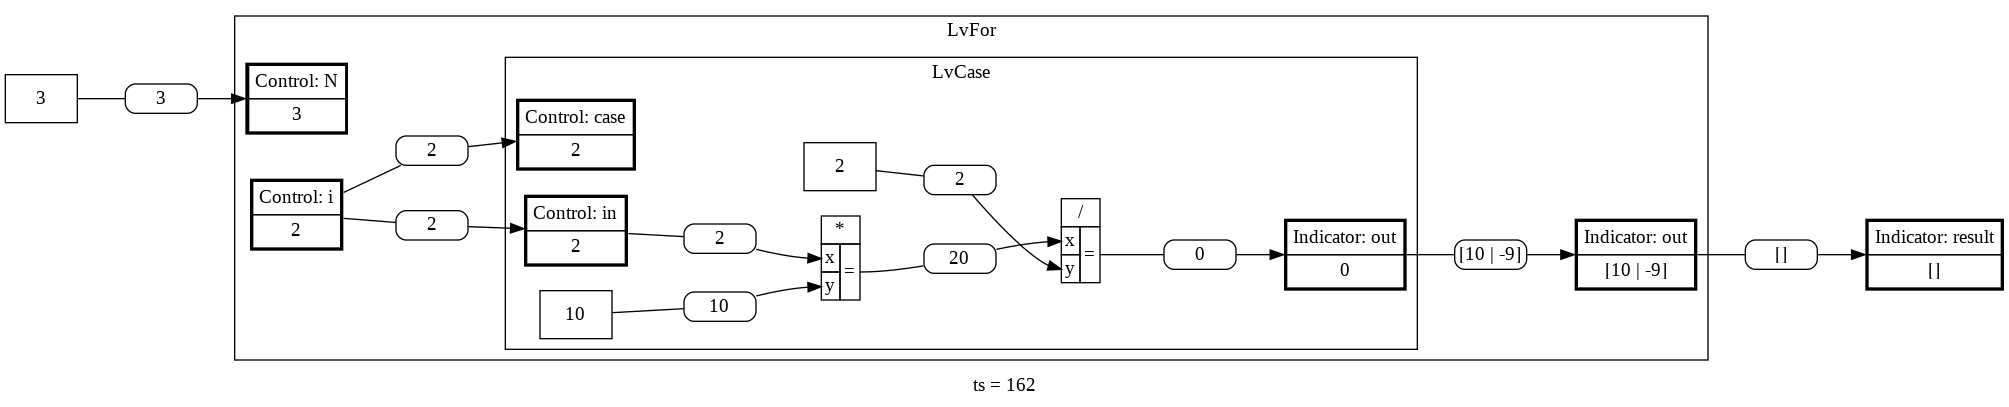
\includegraphics[width=0.99\columnwidth]{lv_graph_example}

\noindent The test program for this example is the following.

../LvInterpreter_demo.tex
